En el capítulo \ref{chap:CR3BP} se estudió el Problema Circular de Tres Cuerpos (PC3C). Dos partículas primarias orbitando en un plano a velocidad constante respecto a su centro de masa y una tercera influenciada por las otras dos con una dinámica muy rica. Es rica por elementos como la sensibilidad al parámetro de masa, dada por la ecuación (\ref{eq:mu_critica}), la sensibilidad a condiciones inciales cercanas, las regiones discriminadas por su constante de Jacobi, o sus cinco puntos lagrangianos. Esta sección busca explotar el Transporte de Jets (JT) como se describe en el capítulo \ref{chap:jt} así como los indicadores y herramientas desarrolladas en \ref{chap:jt_indicators}.


Este capítulo se divide como sigue: La sección \ref{sec:parametrization} parametriza a $\mu$ y hace un TJ de dicha parametrización. La sección \ref{sec:asteroids} estudia la probabilidad de colisión entre dos asteroides orbitando cerca de la Tierra. Luego, en \ref{sec:C3BP_simplecticity} se estudia la simplecticidad del PC3C. Finalmente, en la sección \ref{sec:C3BP_heatmaps} se presentan los campos escalares y vectoriales de $\xi_{max}$ y $\theta_{\pm}$ y se compara con los resultados para el campo de ELTF.

\section{Parametrización de $\mu$}
\label{sec:parametrization}

Como se analizó en la sección \ref{sec:lag_points}, $L_i = L_i(\mu)$, es decir, los puntos de equilibrio del PC3C dependen todos del parámetro de masa del sistema. Los puntos $L_4(\mu)$ y $L_5(\mu)$ son de particular interés ya que, a diferencia de los otros tres, serán estables si $\mu \leq \mu_c$, donde $\mu_c$ es el parámetro crítico de la masa dado por (\ref{eq:mu_critica}). 

El análisis de eigenvalores alrededor de los puntos singulares nos da cómo es la estabilidad de dichos puntos. Sin embargo, es interesante ver las soluciones cerca de $\mu_c$ ya que nos permitirá ver directamente en el flujo el comportamiento de estabilidad de la partícula que visita a $L_4$ o $L_5$.

Para esto, se seguirá la filosofía de la sección \ref{sec:parameter_variation}, donde se agregará a las ecuaciones de movimiento la ecuación 
\begin{equation*}
 \dot{\mu} = 0
\end{equation*}
y se hará un TJ en $\mu$, es decir, ésta se parametrizará como 
\begin{equation*}
 \mu = \mu_0 + \delta\mu,
\end{equation*}   
donde $\delta\mu \in \pkM$ y, por tanto, $\mu \in \pkM$ también. Se introduce la notación $\phi_\mu(t;t_0,\xo)$ para referirse a este tipo de transporte. Tomando $\mu_0 = \mu_c \approx 0.0385$, se está en el límite entre la estabilidad y la divergencia alrededor de los puntos $L_4$ y $L_5$.

%FIGURA!
\begin{figure}
 \centering
 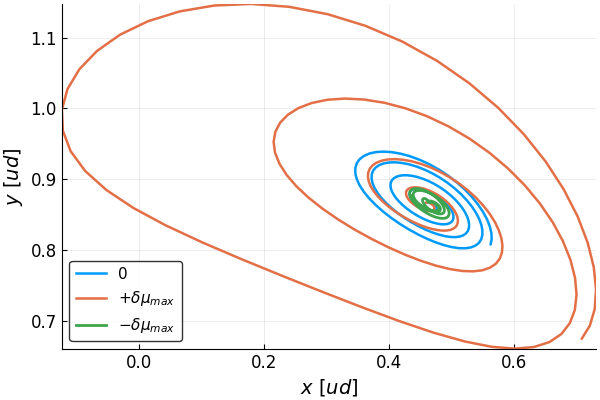
\includegraphics[width=0.8\linewidth]{flow_dmu}
 \caption{Espacio de configuraciones para $\phi_\mu$ con variaciones $\delta\mu = 0$ (azul), $\delta\mu = \delta\mu_{max}$ (naranja), y $\delta\mu = -\delta\mu_{max}$ (verde), donde $\delta\mu_{max} = \xi_{max}(\phi_\mu) \approx 0.00329$. Para el transporte se usó un jet de orden $M=18$ con condiciones iniciales $\left( L_{4_x}, L_{4_y} + \Delta y, 0, 0, \mu \right)$.}
 \label{fig:flow_dmu}
\end{figure}

Para el transporte, tomaremos como condición inicial a $\xo = \left( L_{4_x}, L_{4_y} + \Delta y, 0, 0, \mu \right)$ con $\Delta y = 7\times 10^{-4}$ para no estar exáctamente en $L_4$. Las variaciones de $\delta\mu$ estarán acotadas por el tamaño máximo de vecindad de la expresión (\ref{eq:ximax}), es decir, $\lvert \delta\mu \rvert \leq \lvert \delta\mu_{max} \rvert = \xi_{max}(\phi_\mu) \approx 0.033$ en este caso. Se puede ver en la Figura \ref{fig:flow_dmu} una integración a $40$ unidades temporales. Se observa cómo para $\delta \mu > 0$, las soluciones se alejan cada vez más de $L_4$, mientras que para $\delta \mu < 0$ se queda en cierta localidad. Una forma de observar este comportamiento de manera más clara es si medimos la separación de $\phi_\mu(t)$ respecto de $\xo$ para distintos valores de $\delta \mu$. La Figura \ref{fig:remoteness_dmu} muestra esta separación en función del tiempo. Se puede observar que mientras mayor sea la variación de $\mu$, mayor es la tendencia y mayor la amplitud de oscilación. 

%FIGURA! 
\begin{figure}
 \centering
 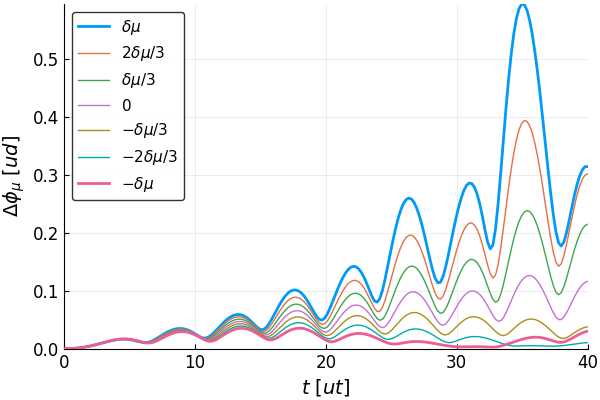
\includegraphics[width=0.8\linewidth]{remoteness_dmu}
 \caption{Diferencia $\Delta\phi_\mu(t) = \norm{ \phi_\mu(t) - \xo }$ del espacio de configuraciones para $\delta\mu \in \left\lbrace -\delta\mu_{max}, -2\delta\mu_{max}/3, -\delta\mu_{max}/3, 0, \delta\mu_{max}/3, 2\delta\mu_{max}/3, \delta\mu_{max}  \right\rbrace$.}
 \label{fig:remoteness_dmu}
\end{figure}

Una forma de ver realmente cuándo el flujo no diverge de la localidad de $L_4$ es si podemos aislar la tendencia de la amplitud de los ciclos. Para esto, se puede usar un filtro de Hodrick-Prescott, que separa una serie de tiempo en tendencia y ciclo. Sea $y_t$ la variable de una serie de tiempo al tiempo $t$. Se asume que dicha serie está compuesta de una componente de tendencia $\tau_t$ más una componente cíclica $c_t$, es decir, $y_t = \tau_t + c_t$\footnote{Normalmente se incluye una componente de error $\eta_t$ que, en este caso, será absorbida por $c_t$.}. Así, uno puede encontrar la tendencia, como se plantea en \cite{Hodrick1997}, bajo el problema de minimización
\begin{equation}
 \min_{\tau} \left( \sum_{t=1}^T (y_t - \tau_t)^2 + \lambda \sum_{t=2}^{T-1} \left[ (\tau_{t+1} - \tau_t) - (\tau_t - \tau_{t-1}) \right]^2 \right),
 \label{eq:hp-filter}
\end{equation} 
con $\lambda$ un parámetro positivo que regula la variabilidad en la componente de tendencia de la serie.

Tomaremos la solución matricial lineal de \cite{Kim2004}  
\begin{equation}
 \mathbf{y}_t = \left( \lambda \mathbf{F} + \mathbf{I}_t \right) \tau_t
 \label{eq:hp_matrix}
\end{equation}  
al derivar (\ref{eq:hp-filter}) respecto a $\tau_t$, donde
\begin{align}
 \mathbf{F} = \left[ \begin{array}{cccccccccc}
 1  & -2 & 1  & 0  & \cdots &        &        & & \cdots & 0    \\
 -2 & 5  & -4 & 1  & 0      & \cdots &        & & \cdots & 0    \\
 1  & -4 & 6  & -4 & 1      & 0      & \cdots & & \cdots & 0    \\
 0  & 1  & -4 & 6  & -4 & 1 & 0      & \cdots &        & \vdots \\
 \vdots  & \ddots  &  &  &  &  &  &  &        & \ddots          \\
    &    &    &  0 &  1 &-4 &    6   & -4     &      1 & 0      \\
   &   &  & \cdots &  0 & 1 &   -4   &  6     &      4 & 1      \\
   &   &  &  &   \cdots & 0 &    1   &  -4    &      5 & 2      \\
 0 &\cdots&  &  &  & \cdots &    0   &   1    &     -2 & 1      \\
 \end{array} \right],
\end{align}

ya que ésta es fácilmente programable. De (\ref{eq:hp_matrix}), obtenemos que $\mathbf{\tau}_t = \left( \lambda \mathbf{F} + \mathbf{I}_t \right)^{-1} y_t$ y $c_t = y_t - \tau_t$. Aplicando este filtro en la Figura \ref{fig:remoteness_dmu}, se obtiene el ciclo y la tendencia tal como se presenta en la Figura \ref{fig:trendcycle_dmu}. En ésta, se observa cómo desde la primera variación negativa ($\delta\mu = -\delta\mu_{max}/3$) hacia valores más negativos, la tendencia decrece después de llegar a un máximo. Esto quiere decir que la distancia respecto al punto inicial no diverge, como se había predicho en el análisis de estabilidad lineal de (\ref{eq:stability_CR3BP}). Por otro lado, es interesante ver cómo la amplitud de las oscilaciones en la parte cíclico de $\Delta\phi_\mu$ son mayores entre mayor sea $\delta_\mu$, ya que muestra cómo aunque la partícula tiende a acercarse a $L_4$, ésta se aleja más cada vez.

%FIGURA!
\begin{figure}[h!]
\centering
\begin{subfigure}{0.49\textwidth}
	\centering
	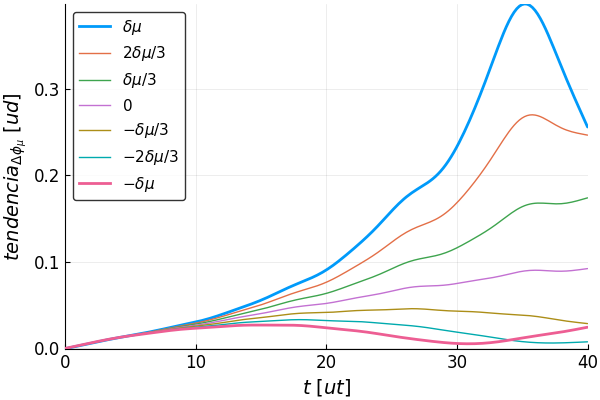
\includegraphics[width = \textwidth]{trends_dmu}
\end{subfigure}
%
\begin{subfigure}{0.49\textwidth}
	\centering
	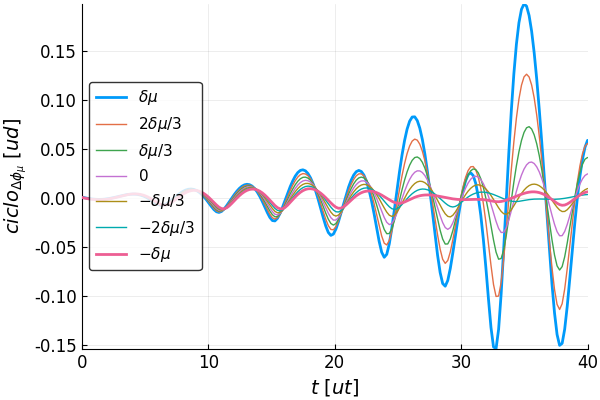
\includegraphics[width = \textwidth]{cycles_dmu}
\end{subfigure}
\caption{ Separación en tendencia (izquierda) y ciclo(derecha) de los valores de la Figura \ref{fig:remoteness_dmu} usando un filtro de Hodrick-Prescott con $\lambda = 8000$.}
\label{fig:trendcycle_dmu}
\end{figure}

Hacer esta separación ayuda fuertemente al análisis de estabilidad de $\mu$ alrededor de $L_4$ y $L_5$ cuando $\mu = \mu_c \pm \delta\mu$, pero ¿seguirán siendo las órbitas en el caso donde $\mu \ll \mu_c$ como en el caso Tierra-Luna?

\subsection{Caso Tierra-Luna}
Dado que en la adimensionalización de las ecuaciones de movimiento el problema queda planteado únicamente en términos de $\mu$, basta ver que en el caso Tierra-Luna $M_T = 5.972 \times 10^{24} \textrm{kg} $, $M_L = 7.348 \times 10^{22} \textrm{kg}$ y, por tanto, $\mu_{TL} = 0.01215$. Notamos que $\mu_{TL} \ll \mu_c$ por lo que alrededor de $L_4$ y $L_5$ debería haber órbitas estables, aún cuando $\delta\mu_{max}$ sea grande.

%FIGURA!
\begin{figure}
 \centering
 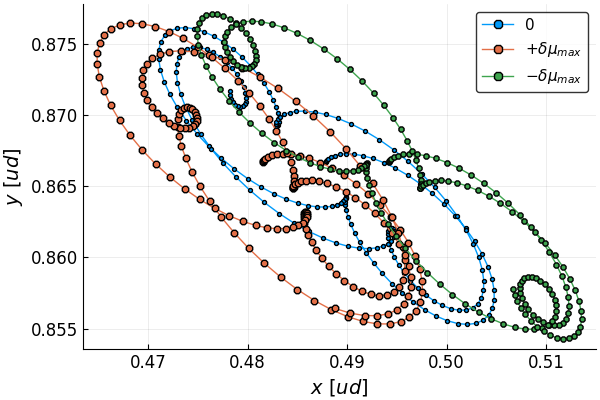
\includegraphics[width=0.7\linewidth]{flow_tl}
 \caption{Espacio de configuraciones para $\phi_\mu$ con variaciones $\delta\mu = 0$ (azul), $\delta\mu = \delta\mu_{max}$ (naranja), y $\delta\mu = -\delta\mu_{max}$ (verde), donde $\delta\mu_{max} = \xi_{max}(\phi_\mu) \approx 0.0063$. Para el transporte se usó un jet de orden $n=18$ con condiciones iniciales $\left( L_{4_x}, L_{4_y} + \Delta y, 0, 0, \mu \right)$.}
 \label{fig:flow_tl}
\end{figure}

Primero, al hacer el Transporte de Jets a $40$ unidades temporales y ver el espacio de configuraciones como se muestra en la Figura \ref{fig:flow_tl}, se observa cómo las tres trayectorias $\delta\mu = \left\lbrace -\delta\mu_{max}, 0, \delta\mu_{max} \right\rbrace$ quedan siempre orbitando alrededor de $L_4$, es decir, no divergen. Resulta que $\delta\mu_{max} = 0.0063 $, lo cual equivale a una variación del $52.14 \%$ respecto a $\mu_{TL}$. Para ponerlo en perspectiva, $\mu_{TL}$ equivale a que la masa primaria (la Tierra) es unas $81$ veces más grande que la secundaria (luna). Así, $\mu_{TL} \pm \delta\mu_{max}$ equivale a que la masa primaria sea $53$ y $171$ veces más grande que la otra, respectivamente. Análogo a la Figura \ref{fig:remoteness_dmu}, la Figura \ref{fig:remoteness_tl} presenta la separación respecto a $\xo$ de la solución. Aquí se puede observar que, aunque al principio (en las primeras $8$ unidades, aproximadamente) las tendencias y oscilaciones siguen el mismo comportamiento que en el caso anterior, éstas se vuelven rápidamente  arbitrarias, sin tener tendencia aparente ni amplitudes crecientes en los ciclos.

%FIGURA!
\begin{figure}
 \centering
 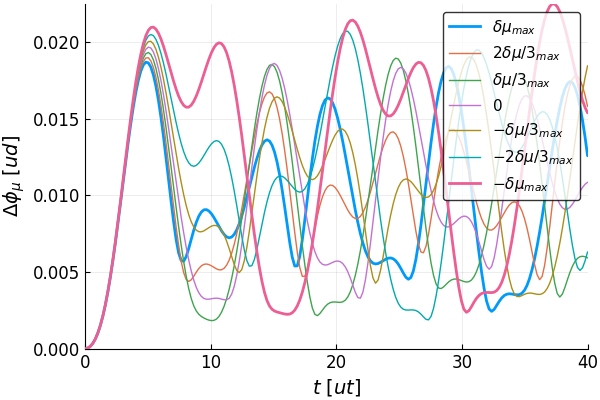
\includegraphics[width=0.7\linewidth]{remoteness_tl}
 \caption{Diferencia $\Delta\phi_\mu(t) = \norm{ \phi_\mu(t) - \xo }$ del espacio de configuraciones para $\delta\mu \in \left\lbrace -\delta\mu_{max}, -2\delta\mu_{max}/3, -\delta\mu_{max}/3, 0, \delta\mu_{max}/3, 2\delta\mu_{max}/3, \delta\mu_{max}  \right\rbrace$ integrado a $40$ unidades temporales.}
 \label{fig:remoteness_tl}
\end{figure}

De hecho, en la Figura \ref{fig:trendcycle_tl} se muestran los gráficas al aplicar el filtro de Hodrick-Prescott. Al aplicar dicho filtro, ¡no se puede observar absolutamente nada! Ni la gráfica de ciclo ni la de tendencia tienen ninguna coherencia en realción a las variaciones del parámetro de masa. Esto significa que $\mu_{TL} + \delta\mu$ es, en efecto, estable para todo el conjunto de valores $\delta\mu$ evaluados alrededor de $L_4$ y $L_5$. Este es un caso donde el TJ es una herramienta natural para evaluar la estabilidad de estos puntos lagrangianos y para ver cómo varían las trayectorias en función de los parámetros del problema-. Muchas otras exploraciones se pueden hacer con variación de parámetros en el problema de tres cuerpos. Sin embargo, este análisis basta para ver las capacidades del TJ cuando no son específicamente ``jets'' los que transporta.

%FIGURA!
\begin{figure}[h!]
\centering
\begin{subfigure}{0.49\textwidth}
	\centering
	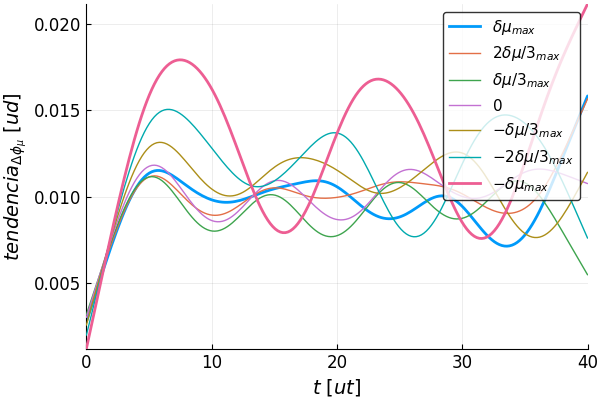
\includegraphics[width = \textwidth]{trends_tl}
\end{subfigure}
%
\begin{subfigure}{0.49\textwidth}
	\centering
	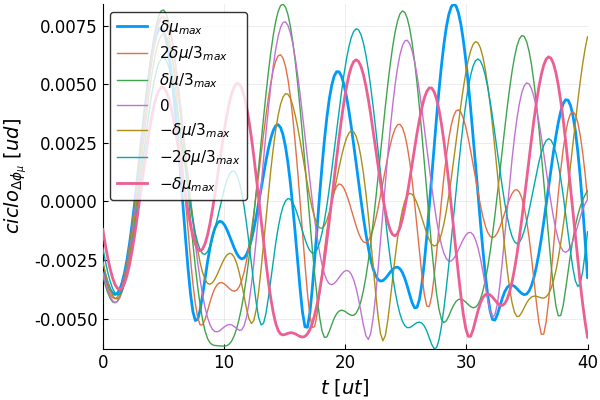
\includegraphics[width = \textwidth]{cycles_tl}
\end{subfigure}
\caption{ Separación en tendencia (izquierda) y ciclo(derecha) de los valores de la Figura \ref{fig:remoteness_tl} usando un filtro de Hodrick-Prescott con $\lambda = 8000$.}
\label{fig:trendcycle_tl}
\end{figure}

\section{Colisión de asteroides}
\label{sec:asteroids}

Sean $a_1$ y $a_2$ dos asteroides con la misma energía de Jacobi alrededor de la Tierra. Éstos se verán afectados únicamente por la atracción gravitacional de la Tierra y la Luna. Esta sección plantea un modelo ilustrativo que permite encontrar la probabilidad de colisión entre $a_1$ y $a_2$, donde los pasos a seguir son similares a los planteados en \cite{Perez2013}. Cabe mencionar que éste es un sistema poco realista ya que, en general, habría que considerar la presencia gravitacional del Sol, la radiación solar, la geometría de los asteroides y demás efectos que influyen en la dinámica de $a_1$ y $a_2$.

Inicialmente, los asteroides se encuentran a $\mathbf{x}_{a_1}(t_0) + \delta\mathbf{x}_{a_1}(t_0)$  y $\mathbf{x}_{a_2}(t_0) + \delta\mathbf{x}_{a_2}(t_0)$, respectivamente, donde $\delta\mathbf{x}_{a_i} \in \pkk{n}{2}$. La variación en cada condición representa el error de medición de éstos. Por tomar una referencia, se tomará la incertidumbre del orden de los datos del asteroide Apophis en los años $2012 - 2028$ \cite{Desmars2013}, donde definimos $\Delta_{max} := 350 $ km como la incertidumbre máxima para los asteroides.

La Figura \ref{fig:asteroid_collision_nominal_integration} muestra la trayectoria nominal de $a_1$ y $a_2$ para condiciones iniciales con energía $C_J = -1.81252 < C_J(L_1)$. En esta integración, la mínima distancia entre ambos cuerpos es de $0.00348$ que representa unos $1341$ kilómetros. Sin embargo, aunque para esta condición particular los asteroides no chocan, es posible que sí lo hagan dentro de una integración con variación hasta de radio $\Delta_{max}$. Esto se puede hacer con el Transporte de Jets de la siguiente manera: 

%FIGURA!
\begin{figure}
 \centering
 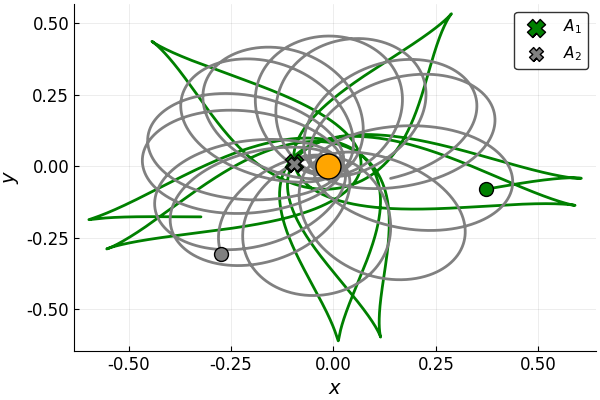
\includegraphics[width=0.7\linewidth]{asteroid_collision_nominal_integration}
 \caption{Integración nominal a $T=10 \approx $ unidades temporales, donde $\mathbf{q}_{a_1}(t_0) = \left( -0.373098, -0.0804321, 1.21995, \dot{y}_{a_1} \left( x_{a_1}(t_0), y_{a_1}(t_0), \dot{x}_{a_1}(t_0), C_J \right) \right)$ 
 y $\mathbf{q}_{a_2}(t_0) = \left( -0.27324, -0.307896, -0.307576, \dot{y}_{a_2} \left( x_{a_2}(t_0), y_{a_2}(t_0), \dot{x}_{a_2}(t_0), C_J \right) \right)$. El círculo naranja representa a $M_1$, y los círculos verde y gris a $\mathbf{q}_{a_1}(t_0)$ y $\mathbf{q}_{a_2}(t_0)$, respectivamente. La zona de mayor acercamiento se marca con cruces, donde en ésta, la distancia entre los asteroides es de $0.00348 \approx 1341$ km.}
 \label{fig:asteroid_collision_nominal_integration}
\end{figure}

\begin{itemize}
 \item Hacer una integración nominal de dos asteroides con energías similares o que se sepa que pueden tener riesgo de colisión.
 
 \item Obtener las coordenadas $\mathbf{q}_{a_i}^{(col)}$ donde la distancia entre $a_1$ y $a_2$ es mínima.
 
 \item Hacer TJ alrededor de las condiciones encontrada en el punto anterior para encontrar la parametrización de la vecindad que pasa por la zona de posible colisión.
 
 \item Encontrar la trayectoria de una distribución de $N$ puntos al evaluar los polinomios en la bola $\delta\mathbf{x}_i \leq \Delta_{max}$ alrededor de $\mathbf{q}_{a_i}^{(col)}$ para ambos asteroides y determinar la distancia entre cada par de puntos.
 
 \item Definir una distancia $D_{col}$ para la cual los asteroides chocarían y determinar qué puntos de la distribución son menores que ésta.
 
 \item Determinar la probabilidad de impacto $\mathcal{P}$ como la cantidad de veces puntos que quedan debajo de $D_{col}$ respecto al número de trayectorias totales $N^2$; así
 \begin{equation} 
 \mathcal{P} = \frac{ \# \left( \norm{\mathbf{x}_{a_1} - \mathbf{x}_{a_2} }    \leq D_{col} \right) }{N^2}.
 \end{equation}
\end{itemize}

%FIGURA!
\begin{figure}
 \centering
 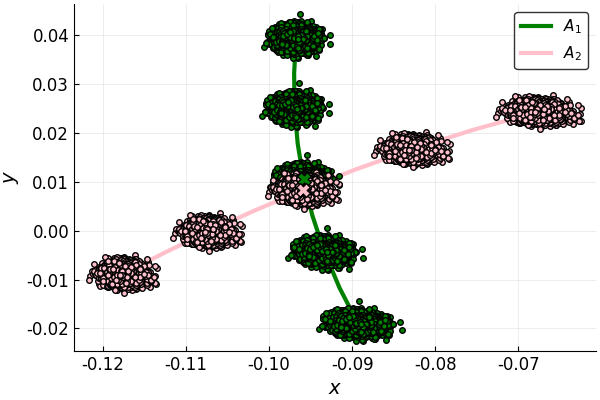
\includegraphics[width=0.7\linewidth]{asteroid_collision_distribution}
 \caption{Transporte de jets de orden $4$ alrededor de $\mathbf{q}_{a_i}^{(col)}$ (cruces en la figura) donde los cúmulos son la distribución de radio $\delta\mathbf{x}_{a_i} \leq 350$ km evaluados en el polinomio resultante del transporte. Para el método sólo se toman los cúmulos donde se encuentran $\mathbf{q}_{a_i}^{(col)}$, pero la figura busca ilustrar una sección de la trayectoria de los asteroides.}
 \label{fig:asteroid_collision_distribution}
\end{figure}

La Figura \ref{fig:asteroid_collision_distribution} muestra una distribución normal de $7000$ puntos\footnote{$ N = 7000$ ya converge a una probabilidad cuyas cifras significativas no afectan el redondeo de la Tabla \ref{table:collision_table}.} evaluados en el transporte alrededor de $\mathbf{q}_{a_i}^{(col)}$ para $i = \{1,2\}$. La probabilidad de impacto dependerá del tamaño que tengan los asteroides, la cual se presenta en la Tabla \ref{table:collision_table}. Se presenta en la Figura \ref{fig:asteroid_collision_histogram} la distribución de distancias entre ambos asteroides en la zona de riesgo de colisión. Aún cuando $D_{col}$ e incluso $\Delta_{max}$ quedan debajo del escenario más posible en la distribución, la probabilidad de impacto es suficientemente grande para no ser ignorada en los asteroides de mayor dimensión.

%TABLA!
\begin{table}[h!]
\centering
\begin{tabular}{c|c|c}
\toprule
\textbf{$ D_{col}$ [ km ]} & \textbf{$\mathcal{P}$ [ $\%$ ]} & \textbf{Colisiones [ $ \# $ ]} \\ \cmidrule(l){1-3} 
\textbf{$0.5$} &   $3.7 \times 10^{-5}$   & $18$          \\
\textbf{$5$}   &   $0.0048$               & $2356$        \\
\textbf{$30$}  &   $0.172$                & $84,609$     \\
\textbf{$150$} &   $4.357$                & $2,135,173$   \\ \bottomrule 
\end{tabular}
\caption{Número de colisiones y riesgo de choque para asteroides de distintas dimensiones.}
\label{table:collision_table}
\end{table}

%FIGURA!
\begin{figure}
 \centering
 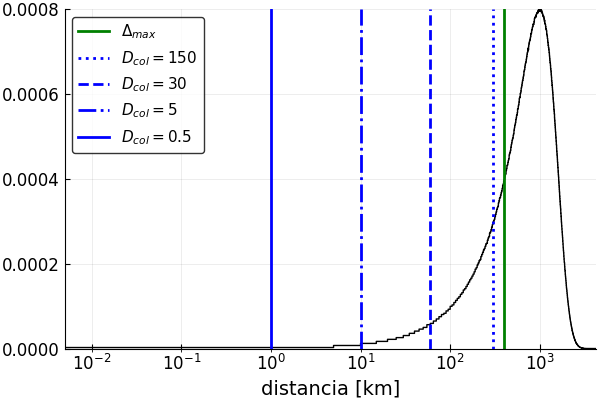
\includegraphics[width=0.7\linewidth]{asteroid_collision_histogram}
 \caption{Distribución normalizada de distancias entre $a_1$ y $a_2$ cerca del punto de posible colisión dadas $7000$ variaciones iniciales alrededor de $\mathbf{q}_{a_1}^{col}$ y $\mathbf{q}_{a_2}^{col}$. Las líneas verticales muestran los valores usados en la Tabla \ref{table:collision_table}.}
 \label{fig:asteroid_collision_histogram}
\end{figure}


Algo relevante al hacer Transporte de Jets es la presición de éste. Se encuentra que $\xi_{max}(\phi_{a_1}) = 0.0022 \approx 865 \ km \gg \Delta_{max}$\footnote{$\xi_{max}(\phi_{a_2})$ es prácticamente igual a $\xi_{max}(\phi_{a_1})$, por lo que sólo se usa $\phi_{a_1})$.}, por lo que se tiene bastante confianza en la precisión de las evaluaciones de la distribución. De hecho, al tomar una serie de variaciones $\norm{\delta\mathbf{x}_{a_i}} = \Delta_{max}$ y hacer la integración nominal de éstas, se encuentra que el error promedio respecto a éstas es del orden de $10^{-11} \approx 4 mm$, o sea, nada. Esto se muestra en la Figura \ref{fig:asteroid_jt_vs_nominal}.

%FIGURA!
\begin{figure}
 \centering
 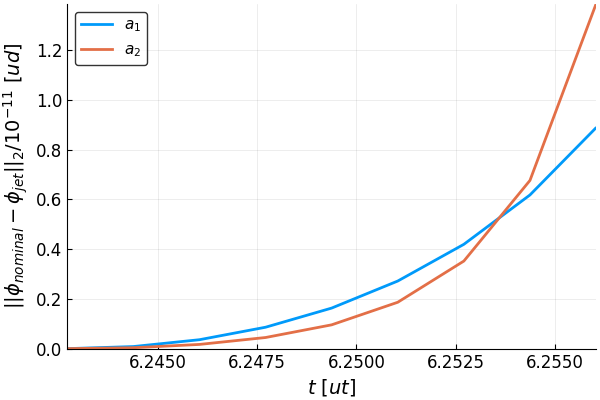
\includegraphics[width=0.7\linewidth]{asteroid_jt_vs_nominal}
 \caption{Promedio de la distancia entre la integración nominal y el TJ para $500$ condiciones iniciales con variación $\norm{\delta\mathbf{x}_{a_1}} = \norm{\delta\mathbf{x}_{a_1}} = \Delta_{max}$.}
 \label{fig:asteroid_jt_vs_nominal}
\end{figure}

Así, ilustramos el método de posible colisión entre asteroides, donde se establece la probabilidad de impacto para diferentes zonas de colisión. El TJ permitió encontrar dichas probabilidades ya que en éste, simplemente hubo que evaluar la distribución de variaciones iniciales en un radio dado. Éste método es generalizable a cualquier sistema donde exista alguna incertidumbre en las condiciones iniciales. Sin embargo, hay que tener claro que el TJ no es muy preciso para integraciones muy largas ni para vecindades muy grandes. En este ejemplo, el radio de las variaciones eran $0.46$ veces más pequeñas que $\xi_{max}$. Además, se hizo la integración de jets cerca del punto de posible colisión para tener tiempo de integración cortos. 

%Mencionar adimensionalización del tiempo para ver cuánto implica 1 unidad temporal.

\section{Simplecticidad del problema circular}
\label{sec:C3BP_simplecticity}

Se construyeron en el capítulo \ref{chap:CR3BP} los potenciales (\ref{eq:3body_potential}) y sus respectivas energías cinéticas (\ref{eq:3body_kinetic}) del problema general de tres cuerpos. Éstas nos permiten definir al hamiltoniano
\begin{equation}
 H(\mathbf{r}_1, \mathbf{r}_2, \mathbf{r}_3, \mathbf{p}_1, \mathbf{p}_2, \mathbf{p}_3) = \sum_{i=1}^3 h_i(r_{i,j}, r_{i,k}, \mathbf{p}_i),
 \label{eq:3BP_hamiltonian}
\end{equation} 
donde $\mathbf{p}_i = M_i \dot{\mathbf{r}}_i$ es el momento conjugado y
\begin{equation}
 h_i(r_{i,j}, r_{i,k}, \mathbf{p}_i) = \frac{1}{2 M_i} p_i^2 + U_{M_i}(r_{i,j}, r_{i,k}),
 \label{eq:individual_hamiltonian}
\end{equation}
los hamiltonianos para cada una de los cuerpos. Notemos que (\ref{eq:3BP_hamiltonian}) no depende del tiempo y, por lo tanto, es un sistema conservativo. 

Cuando en la sección \ref{sec:R3BP} se supuso que la masa menor no influye en la dinámica de las masas primarias, bastó con hacer una rotación con velocidad angular $\Omega$ para encontrar las ecuaciones de movimiento de $m_3$. Esto fija las masas primarias, cancela sus hamiltonianos ($  U_{M_2} = - U_{M_1}$) y define al hamiltoniano para la masa menor. Dicha rotación se puede realizar bajo el cambio de coordenadas
\begin{align*}
 x &= X\cos (\Omega t) - Y \sin (\Omega t), \\
 y &= X\sin (\Omega t) - Y \cos (\Omega t), 
\end{align*} 
con $(x,y)$ y $(X,Y)$ las nuevas y viejas coordenadas para $m_3$, respectivamente, tal como se muestra en la Figura \ref{fig:rotating_frames}.

%FIGURA!
\begin{figure}[h!]
 \centering
 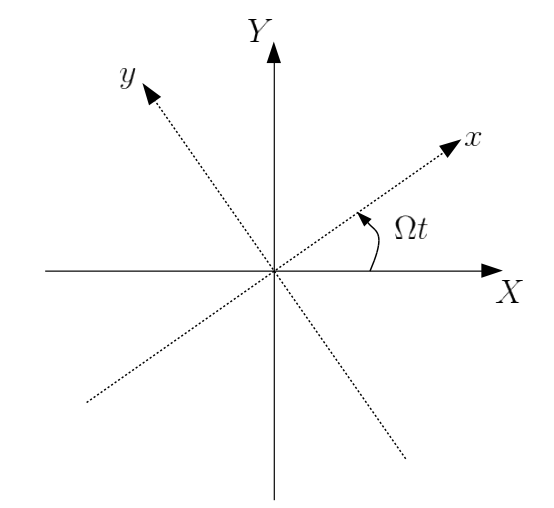
\includegraphics[scale=0.52]{rotating_frame}
 \caption{Diagrama del cambio de marco de referencia $(X,Y)$ a $(x,y)$ a velocidad angular $\Omega$.}
 \label{fig:rotating_frames}
\end{figure}

Para obtener el hamiltoniano modificado, que a veces en la literatura literatura se llama kamiltoniano \cite{Goldstein2007, Johns2011}, es necesario ver cómo se modifica el momento conjugado en el nuevo sistema donde, para esto, se debe conservar el principio de mínima acción

\begin{align}
 \delta \int_{t_0}^t \left( \dot{\mathbf{R}} \cdot \mathbf{P} - H(\mathbf{R}, \mathbf{P}, \tau) \right) d\tau &= 0 \nonumber \\
\implies \delta \int_{t_0}^t \left( \dot{\mathbf{r}} \cdot \mathbf{p} - K(\mathbf{r}, \mathbf{p}, \tau) \right) d\tau &= 0
 \label{eq:kamiltonian_condition}
\end{align}
en ambos ejes, lo cual sucede si
\begin{equation}
 \dot{\mathbf{R}} \cdot \mathbf{P} - H(\mathbf{R}, \mathbf{P}) = \dot{\mathbf{r}} \cdot \mathbf{p} - K(\mathbf{r}, \mathbf{p}, t) + \frac{dG(\mathbf{R}, \mathbf{p}, t)}{dt}.
\end{equation}
Aquí $\mathbf{P} = (P_x,P_y)$, $\mathbf{R} = (X,Y)$, $\mathbf{p} = (p_x,p_y)$, $\mathbf{r} = (x,y)$, $K$ es el kamiltoniano y $G = - \mathbf{r} \cdot \mathbf{p} + G_2(\mathbf{R}, \mathbf{p}, t)$ es una función que genera una transformación canónica entre ambos sistemas, también conocida como función generatriz de tipo 2 \cite{CanonicalTransformations}. Notemos que como 
\begin{align*}
 \frac{dG}{dt} =  - \dot{\mathbf{r}}\cdot \mathbf{p} - \mathbf{r}\cdot \dot{\mathbf{p}} + \pder{G_2}{\mathbf{R}}\dot{\mathbf{R}} + \pder{G_2}{\mathbf{p}}\dot{\mathbf{p}} + \pder{G_2}{t},
\end{align*}
entonces
\begin{align}
 \mathbf{P} &= \pder{G_2}{\mathbf{R}} \nonumber, \\
 \mathbf{r} &= \pder{G_2}{\mathbf{p}} \nonumber, \\
 \therefore K(\mathbf{r}, \mathbf{p}) &= H(\mathbf{r}, \mathbf{p}) + \pder{G_2}{t} (\mathbf{r}, \mathbf{p}).
 \label{eq:kamiltonian_formulae}
\end{align}

Definimos $G_2$ simplemente como
\begin{equation}
 G_2(\mathbf{R}, \mathbf{p}, t) = p_x \underbrace{\left( X \cos (\Omega t) - Y \sin (\Omega t) \right) }_{x} + p_y (\underbrace{ \left( X \sin (\Omega t) + Y \cos (\Omega t) \right)}_{y}
 \label{eq:generating_function}
\end{equation}

y, con (\ref{eq:kamiltonian_formulae}), permite formular explícitamente al kamiltoniano como
\begin{equation*}
 K(\mathbf{r}, \mathbf{p}) = \underbrace{ \frac{1}{2M_3}\left( p_x^2 + p_y^2 \right) - G \frac{M_1}{r_{1,3}} - G \frac{M_2}{r_{2,3}}}_{H(\mathbf{r}, \mathbf{p}) } + \underbrace{\Omega\left( p_y x - p_x y \right) }_{\pder{G}{t}(\mathbf{r}, \mathbf{p})}
\end{equation*}

\begin{equation}
 \therefore K = \frac{1}{2M_3} \left( (p_x - \Omega y)^2 + (p_y + \Omega x)^2 \right) - \left(G \frac{M_1}{r_{1,3}} + G \frac{M_2}{r_{2,3}} + \frac{\Omega^2}{2}\left( x^2 + y^2 \right) \right).
 \label{eq:kamiltonian}
\end{equation}

Notemos que $K = k_3$, así que la partícula menor define al hamiltoniano del sistema en el nuevo sistema de referencia. Ésta nos permite probar numéricamente la propiedad simpléctica del PC3C que, contruido de otro modo, no hubiese sido evidente. Basta con hacer las transformaciones 
\begin{align}
p_x &\to p_x - \Omega y, \\
p_y &\to p_y + \Omega x,
\label{eq:momentum_transformation}
\end{align} 
y aplicar la relación (\ref{eq:sympletic_flow}).

%FIGURA!
\begin{figure}[h!]
\centering
\begin{subfigure}{0.49\textwidth}
	\centering
	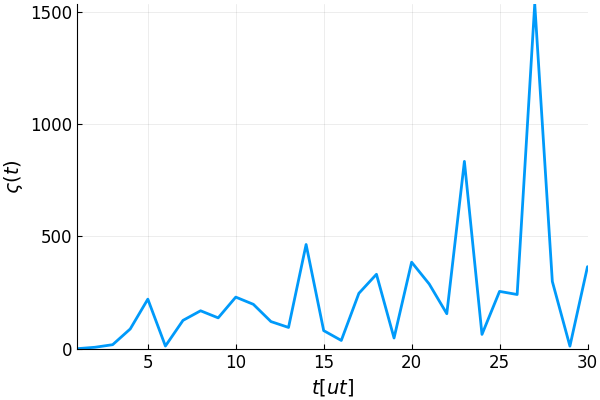
\includegraphics[width = \textwidth]{non_symplectic_L1}
\end{subfigure}
%
\begin{subfigure}{0.49\textwidth}
	\centering
	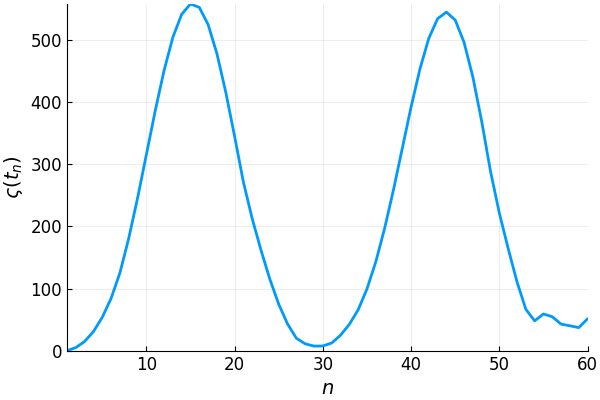
\includegraphics[width = \textwidth]{non_symplectic_L4}
\end{subfigure}
\caption{ $\varsigma(t)$ para $\phi(t)$ sin modificar el flujo en unidades adimensionales del PC3C. Las condiciones iniciales son $\xo = \left( \left( L_{1_x}, 0.001, 0, 0 \right)^T + \delta \xi \right) $ (izquierda) y $ \xo = \left( \left( L_{4_x}, L_{4_y} + 0.001, 0, 0 \right)^T + \delta \xi \right) $ (derecha) para $\delta \xi$ un polinomio de orden $3$.}
\label{fig:non_symplectic_L4_L1}
\end{figure}

Si uno no hace dichas transformaciones, parecerá que el problema no conserva la forma simpléctica, tal como en el ingenuo intento que se muestra en la Figura \ref{fig:non_symplectic_L4_L1} para diferentes condiciones iniciales. Para obtener $\varsigma$ se utiliza la ecuación (\ref{eq:scalar_symplecticity}) que, como se discute en la sección \ref{sec:formas-simplecticas}, opera de manera muy natural con el TJ, ya que la parametrización de vecindades del espacio fase permite computar al jacobiano en cada punto de manera directa.

La Figura \ref{fig:symplectic_L4_L1}, en cambio, muestra la conservación simpléctica del PC3C bajo la transformación (\ref{eq:momentum_transformation}), donde se observa cómo $\varsigma(t)$ se mantiene constante durante toda la integración. En ésta, se tomaron las mismas dos condiciones iniciales que en la Figura \ref{fig:non_symplectic_L4_L1}; una cerca de $L_4$, que es una trayectoría estable, y otra cerca de $L_1$, que orbita alrededor de la masa primaria menor. Se puede observar cómo en la condición más estable la conservación de la simplecticidad varía en unos dos órdenes de magnitud menos que cerca de $L_1$. Sin emabrgo, ambas tienen variaciones menor a $10^{-10}$ en cada punto de la trayectoria, por lo que podemos decir que, en efecto, el sistema es simpléctico. Ésta es una aplicación muy directa para el TJ que aprovecha su estructura paramétrica, de la cual se pueden obetener el jacobiano o incluso variaciones de órdenes mayores. 

%FIGURA!
\begin{figure}[h!]
\centering
\begin{subfigure}{0.49\textwidth}
	\centering
	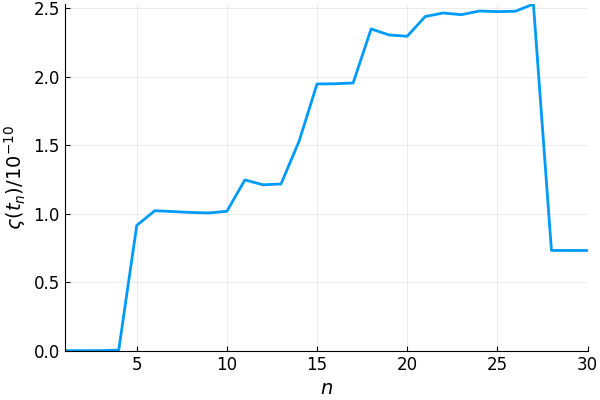
\includegraphics[width = \textwidth]{symplectic_L1}
\end{subfigure}
%
\begin{subfigure}{0.49\textwidth}
	\centering
	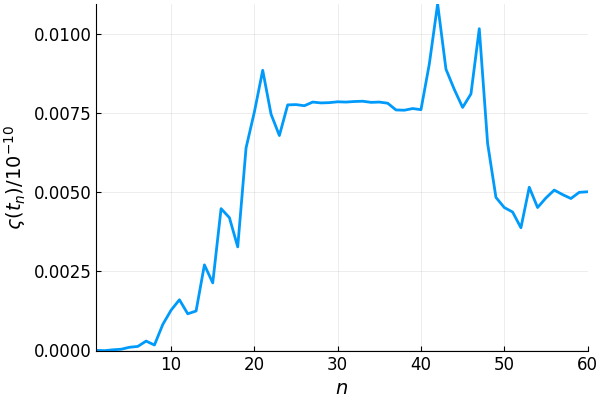
\includegraphics[width = \textwidth]{symplectic_L4}
\end{subfigure}
\caption{$\varsigma(t)$ para $\phi(t)$ con las transformaciones (\ref{eq:momentum_transformation}). Las condiciones iniciales son $\xo = \left( \left( L_{1_x}, 0.001, 0, 0 \right)^T + \delta \xi \right) $ (izquierda) y $ \xo = \left( \left( L_{4_x}, L_{4_y} + 0.001, 0, 0 \right)^T + \delta \xi \right) $ (derecha) para $\delta \xi$ un polinomio de orden $3$.}
\label{fig:symplectic_L4_L1}
\end{figure}

%Valdrá la pena hacer un análisis simpléctico de mayor dimensión?

\section{Campos de $\xi_{max}$ y $\varsigma_\pm$ para el problema circular}
\label{sec:C3BP_heatmaps}

El estudio y exploración del TJ ha utilizado la ecuación (\ref{eq:ximax}) en varias ocaciones hasta ahora. Ésta ha sido el parámetro que nos ha permitido saber qué tan grandes pueden ser las vecindades dado cierto error $\epsilon_{jet}$, tal como se discute en la sección \ref{sec:ximax}. Éste se utilizó en la sección \ref{sec:asteroids} para comprobar que la incertidumbre de medición diera resultados precisos al evaluar la distribución de puntos, y en \ref{sec:parametrization} para las variaciones del parámetro de masa y analizar la estabilidad de $L_4$. $\xi_{max}$ percibe, en esencia, qué tan compleja es la deformación de la vecindad y qué tanto se alejan las condiciones vecinas de la condición nominal a tiempo fijo, por lo que $\xi_{max} \ll 1$ implica una alta sensibilidad en las condiciones iniciales cercanas o un gran gradiente de velocidades para la vecindad. 

%FIGURA! 
\begin{figure}
 \centering
 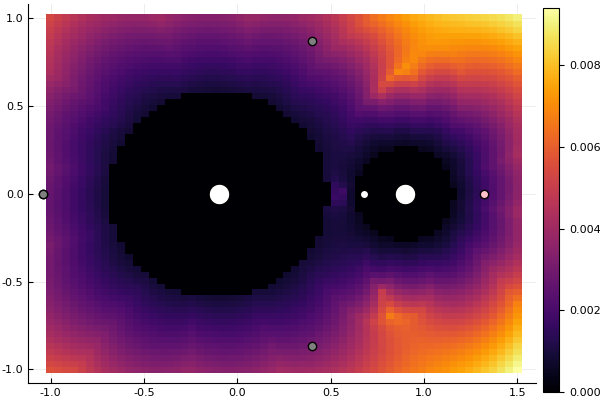
\includegraphics[width=0.7\linewidth]{C3BP_ximax1}
 \caption{Campo escalar de los tamaños máximos de vecindad $\xi_{max}$ en una retícula de $70 \times 70$  después de $0.3$ unidades adimensionales de tiempo en el espacio de configuraciones del PC3C con $\mu = 0.1$. Éste se calculó con tolerancia $\epsilon_{Taylor} = 10^{-7}$, orden de jets $M = 2$ y orden máximo de la expansión $N = 20$. Las condiciones del PC3C son para $\xo = (x_{0_i}, y_{0_j}, 0, 0)^T$, con $x_{0_i} \in (-1, 1.5)$, $y_{0_j} \in (-1, 1.5)$.}
 \label{fig:C3BP_ximax1}
\end{figure}


Para esta sección se hará un análisis del PC3C de los campos escalares de $\xi_{max}$ así como las tasas de expansión y contracción discutidas en \ref{sec:contraccion_expansion} con la misma intención que se hace en \cite{Perez2015}. Dichos campos son comparables con el campo de ELTF desarrollado al principio del capítulo \ref{chap:jt_indicators}, por lo que se hará una comparación con éstos al final de la sección. En el problema restringido el gradiente apunta siempre hacia las masas primarias del sistema, lo cual se puede observar en la Figura \ref{fig:C3BP_ximax1}, donde se calcula el campo escalar para $\xi_{max}$ a $T = 0.3$ unidades adimensionales. Ésta es similar a la representación de curvas de nivel de la Figura \ref{fig:3body_pseudo_potential} de la sección \ref{sec:lag_points} y, al tener un tiempo de integración muy corto, no da tiempo a una gran deformación de las vecindades, planteando únicamente los lugares de mayor gradiente de velocidad. En todas las figuras que se presentan se ignoraron los puntos muy cercanos a las masas primarias, ya que el tiempo de cómputo es muy grande cerca de éstos. 

%FIGURA! 
\begin{figure}
 \centering
 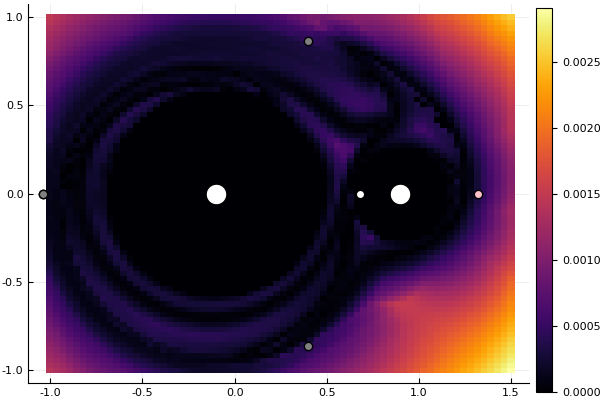
\includegraphics[width=0.7\linewidth]{C3BP_ximax3}
 \caption{Campo escalar de los tamaños máximos de vecindad $\xi_{max}$ con condiciones idénticas que para la Figura \ref{fig:C3BP_ximax1} pero integrado a $3$ unidades temporales.}

 \label{fig:C3BP_ximax3}
\end{figure}

La Figura \ref{fig:C3BP_ximax3}, en cambio, presenta el mismo campo escalar pero integrada a $T = 3$ unidades adimensionales. Como se menciona al inicio de esta sección, las dos principales formas en las que $\xi_{max}$ sea chica es si el gradiente de velocidades en una vecindad es muy grande o si la deformación de la vecindad inicial es muy pronunciada. Ambas figuras muestran cómo $\xi_{max}$ decrece gradualmente al aumentar el gradiente de velocidad hacia las singularidades. Esto muestra la tendencia de la tercer partícula atrayéndose hacia las masas primarias. Sin embargo, en la Figura \ref{fig:C3BP_ximax3} se observan curvas donde $\xi_{max}$ es pequeña  respecto a los valores vecinos. Los puntos en estas curvas, a las cuales llamaremos $\mathcal{C}_s$, no reflejan un gran gradiente de velocidad pero sí una deformación muy pronunciada del jet. Aquí seguramente divergieron las condiciones por debajo y por arriba de la condición inicial. Notemos que el campo planteado en estas figuras tiene una variación $\lvert \xi \rvert \leq \xi_{max}$ en cualquier dirección arbitraria, la cual no corresponde necesariamente a variaciones con la misma energía de Jacobi, por lo que no se puede concluir que las curvas $\mathcal{C}_s$ correspondan a curvas con cantidades conservadas.

%FIGURE!
\begin{figure}
 \centering
 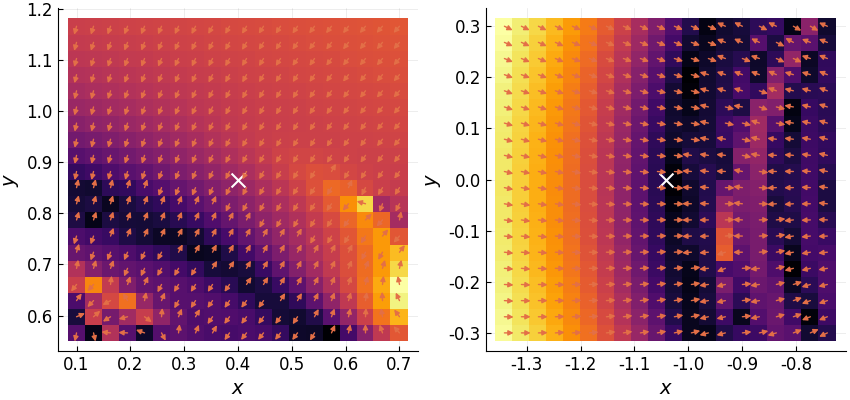
\includegraphics[width=1.0\linewidth]{C3BP_seprate}
 \caption{Campos vectoriales dados por $\left( \cos(\theta_{+}(\xo), \sin(\theta_{+}(\xo) \right)^T$ sobre los campos escalares $\varsigma_{+}(\xo)$ en una cuadrícula de $20 \times 20$, con tolerancia $\epsilon_{Taylor} = 10^{-20}$, orden de los jets $M=2$ y orden del desarrollo de Taylor $N = 25$ integrado a $T = 3$ unidades adimensionales. Las condiciones del PC3C son para $\xo = (x_{0_i}, y_{0_j}, 0, 0)^T$ con $\mu = 0.1$. A la izquierda se observan los puntos cerca de $L_4$, marcada con $\times$, mientras que a la izquierda se presentan las localidades de $L_3$.}
 \label{fig:C3BP_seprate3}
\end{figure}

Para reforzar este análisis, se calcularon las direcciones de mayor expansión para la vecindad de los puntos lagrangianos. La Figura \ref{fig:C3BP_seprate3} presenta dichas direcciones en distintas secciones del espacio de configuraciones, donde se observa cómo en las zonas de menor expansión, equivalentes a las zonas donde $\xi_{max}$ es pequeña,  $\theta_{+}$ cambia drásticamente. Esto nos pensar que dichas curvas pueden ser variedades invariantes en el espacio extendido de las fases, ya que parecen depender del tiempo. Esta figura presenta una acercamiento alrededor de $L_4$ y $L_3$, donde se observa cómo la dirección de  $\theta_{+}$ cambia cuando se cruza por una curva $\mathcal{C}_s$. Lejos de las singularidades el gradiente tiende hacia ellas pero al cruzar por estas curvas especiales, la dirección de expansión máxima cambia de sentido. Se puede inferir que éstas determinan las regiones donde las trayectorias escapan de sus órbitas después de un tiempo dado.

%FIGURE!
\begin{figure}
 \centering
 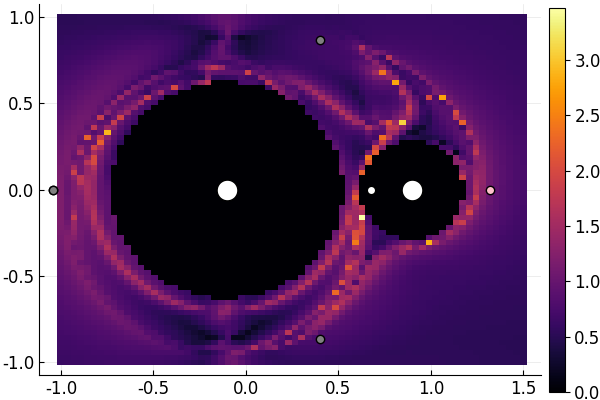
\includegraphics[width=0.7\linewidth]{C3BP_FTLE}
 \caption{Campo escalar dado por los ELTF. Las condiciones y la retícula para esta figura son idénticas a las de \ref{fig:C3BP_ximax3}.}
 \label{fig:C3BP_FTLE}
\end{figure}

Notemos de la Figura \ref{fig:C3BP_FTLE}, que el campo escalar para $\xi_{max}$ es bastante similar al campo de los ELTF. Se presentan las mismas líneas invariantes que en \ref{fig:C3BP_ximax3}. Sin embargo, la diferencia conceptual es que en el caso de ELTF éstas representan las zonas de mayor tasa de expansión, mientras que en $\xi_{max}$ representan el tamaño donde las variaciones son más pequeñas.